% Mobile-C Library 

%%%%%%%%%%%%%%%%%%%%%%%%%%%%%%%%%%%%%%%%%%%%%%%%%%%%%%%%%%%%%%%%%%%%%%
% Preamble {{{
%\documentclass[11pt]{article}
\documentclass[11pt]{report}
\usepackage{varioref}
\usepackage{times,verbatim,fancyheadings,makeidx}
\usepackage{moreverb}
%\usepackage{psfig}
\usepackage[pdftex]{hyperref}
\usepackage{hypcap}
\usepackage{fullpage}
\usepackage{amssymb,amsmath}
\usepackage{graphicx}
\usepackage{program}
%\headrulewidth 0.0pt
%\hoffset=-0.0625in
%\voffset=0pt
\setlength{\textheight}{9in}
\setlength{\textwidth}{6.5in}
\topmargin=0.05in
\makeindex
% }}} Preamble
%%%%%%%%%%%%%%%%%%%%%%%%%%%%%%%%%%%%%%%%%%%%%%%%%%%%%%%%%%%%%%%%%%%%%%

%%%%%%%%%%%%%%%%%%%%%%%%%%%%%%%%%%%%%%%%%%%%%%%%%%%%%%%%%%%%%%%%%%%%%%
% Title Page {{{
\begin{document}
\thispagestyle{empty}
\begin{center}
%\includegraphics[width=1.8in]{figure/mobilec_logo.png}


\vspace{0.5in}
{\Huge\sf\bf User's Guide for Programming iMobot} \\
\vspace{2.0in}
{\large\sf\bf\today}
%September 20, 2007
\end{center}

\pagebreak
% }}} Title Page
%%%%%%%%%%%%%%%%%%%%%%%%%%%%%%%%%%%%%%%%%%%%%%%%%%%%%%%%%%%%%%%%%%%%%%

%%%%%%%%%%%%%%%%%%%%%%%%%%%%%%%%%%%%%%%%%%%%%%%%%%%%%%%%%%%%%%%%%%%%%%
% Abstract {{{
%\phantomsection
%\addcontentsline{toc}{chapter}{Abstract}
\begin{abstract} 
This user's guide describes how to control an iMobot robotic module. The iMobot
robotic module has four controllable degrees of motion. Each module has two
articulated body joints and two rotating faceplates at the ends of the module.
\end{abstract}
\pagebreak
% Abstract }}}
%%%%%%%%%%%%%%%%%%%%%%%%%%%%%%%%%%%%%%%%%%%%%%%%%%%%%%%%%%%%%%%%%%%%%%

%%%%%%%%%%%%%%%%%%%%%%%%%%%%%%%%%%%%%%%%%%%%%%%%%%%%%%%%%%%%%%%%%%%%%%
% Table of Contents {{{
\pagenumbering{roman}
\setcounter{page}{1}
\tableofcontents
\pagebreak
% }}} Table of Contents
%%%%%%%%%%%%%%%%%%%%%%%%%%%%%%%%%%%%%%%%%%%%%%%%%%%%%%%%%%%%%%%%%%%%%%

%%%%%%%%%%%%%%%%%%%%%%%%%%%%%%%%%%%%%%%%%%%%%%%%%%%%%%%%%%%%%%%%%%%%%%
% Part 1 {{{
\pagenumbering{arabic}
\setcounter{page}{1}
\pagebreak
% }}} Part 1 
%%%%%%%%%%%%%%%%%%%%%%%%%%%%%%%%%%%%%%%%%%%%%%%%%%%%%%%%%%%%%%%%%%%%%%

%%%%%%%%%%%%%%%%%%%%%%%%%%%%%%%%%%%%%%%%%%%%%%%%%%%%%%%%%%%%%%%%%%%%%%
% Introduction {{{
%\pagenumbering{arabic}
%\setcounter{page}{1}
%\pagestyle{fancy}
%\section{Introduction}
%\pagebreak
% }}} Introduction
%%%%%%%%%%%%%%%%%%%%%%%%%%%%%%%%%%%%%%%%%%%%%%%%%%%%%%%%%%%%%%%%%%%%%%
\chapter{iMobot Module Orientation}
The iMobot robotic module is a robotic system consisting of four controllable joints. Two
of the joints are articulated body joints, each cabable of rotating 180 degrees. The other
two joints are rotating faceplates located at either end of the module which are able to
freely rotate like wheels. A diagram of the iMobot's joints and positive directions can
be seen in Figure \ref{fig:joint_diagram}.

\begin{figure}
\begin{center}
\includegraphics[width=3.5in]{images/joint_diagram.png}
\caption{\label{fig:joint_diagram}An iMobot module's four joint locations and directions.}
\end{center}
\end{figure}

\chapter{Logging in to the iMobot via WIFI}
\section{Getting Started}
This short guide will enable you to run the provided demo program,
``simple.cpp'', on the iMobot.
\begin{enumerate}
\item Download and install a VNC client
  \begin{itemize}
  \item For Windows, you may download and install TightVNC from \texttt{http://www.tightvnc.com}.
  \item For Mac OS X, you may download and install Chicken of the VNC from\\
  \texttt{http://sourceforge.net/projects/cotvnc/}
  \end{itemize}
\item Log in to the imobot with a VNC client. Most VNC software will come with
both a "client" program and also a "server" or "host" program. When starting
your VNC program, please ensure that you are starting the "client" program and
not the "server" or "host" program.
\item Connect to the iMobot with your VNC client. The default address of the iMobot is \texttt{192.168.0.123}.
\item Open and execute the demo program.
  \begin{enumerate}
  \item Copy the demo program to your home directory with the command\\
  \texttt{cp /usr/local/ch/package/chimobot/demos/simple.cpp \textasciitilde/}
  \item Open the demo program with ChIDE. You may left click on the desktop to open the menu, and select \texttt{Applications -> Accessories -> ChIDE}.
  \item Click on \texttt{File -> Open} within ChIDE and open the program, \texttt{simple.cpp}. 
  \item Click on the ``Run'' button, located near the top right of the ChIDE Window. The robot should now run the program.
  \end{enumerate}
\end{enumerate}

\section{Graphical Control Interface}
\begin{figure}
\begin{center}
\includegraphics[width=3in]{images/imobot_gui_splash.png}
\caption{\label{fig:gui_splash}The iMobot Graphical Control Interface introductory dialog.}
\end{center}
\end{figure}

The iMobot comes with a graphical control interface for controlling the iMobot.
The control interface is able to perform simple locomotion tasks, and can be
used to determine the joint angles of the iMobot. 

The graphical interface can be found in the application menu of the iMobot. Once
a VNC connection to the iMobot has been established, simply left click on the
desktop to bring up the menu, and select the item \texttt{Applications ->
Accessories -> iMobot Controller}. When the controller starts, you will be 
presented with an introductory dialog as shown in Figure \ref{fig:gui_splash}.
This dialog allows you to choose if you wish to connect to a remote module
via Bluetooth, or if the program is currently running on the module you wish
to control. Select the second option, which specifies that the gui is already
running on an iMobot that you wish to control.
 Ensure that 
the application is connected by ensuring that the status bar at the bottom of the
application displays ``Connected''. 

\begin{figure}
\begin{center}
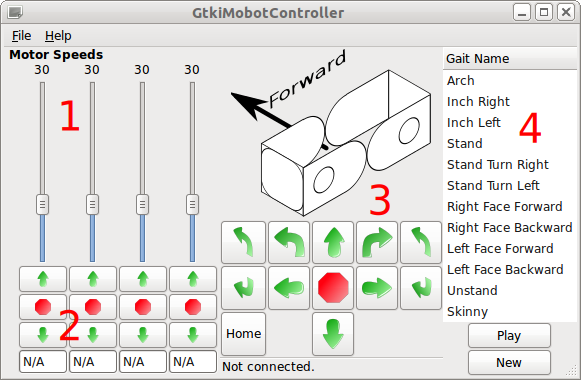
\includegraphics[width=4in]{gui_screenshot.png}
\caption{\label{fig:gui}The iMobot Graphical Control Interface.}
\end{center}
\end{figure}

The graphical interface is composed of four basic components, as shown in
Figure \ref{fig:gui}. The first section, labeled with the red ``1'',
is a section of four sliders. Each slider controls the motor speed of a joint.

The next section, labeled ``2'', are controls which can be used to move each
joint independantly. The upward arrows indicate forward rotation, the stop
buttons stop the motors, and the downward arrows indicate backward motion.
Below the downward arrows are textboxes which display the current angle of each
joint.

The next section, labeled ``3'', contain buttons used for moving the iMobot. 
The arrows indicate forwards and backwards motion, along with turning and
sideways inchworming motions. The large stop sign button stops all motions
on the iMobot. The button labeled ``Home'' causes the iMobot to move all joints
back to their home position. 

The final section, labeled ``4'', contain preprogramed gaits for the iMobot.
To execute a gait, simply select the desired gait by left-clicking on its name,
and click the ``Play'' button.

%%%%%%%%%%%%%%%%%%%%%%%%%%%%%%%%%%%%%%%%%%%%%%%%%%%%%%%%%%%%%%%%%%%%%%
% SUB: Overview of Sample Application Programs {{{
\section{Overview of a Sample Application Program}
The following program is a simple program which moves some joints on the iMobot
before initializing the robot to listen for incoming Bluetooth commands.
\subsection{simple.cpp \label{subsec:simple.cpp}}
\listinginput{1}{../libimobot/Demos/simple_cpp/simple.cpp}
\subsection{Explanation of simple.cpp}
\begin{itemize}
\item 
\begin{verbatim}
  CiMobot robot;
\end{verbatim}
This line declares the \texttt{robot} object, which represents the
capabilities of the iMobot module. This object contains various member
functions which may be executed by the user.
\item 
\begin{verbatim}
  robot.poseZero();
  robot.moveWait();
\end{verbatim}
These commands command the iMobot to move all motors to their zero positions
and wait until the motion is finished.
\item 
\begin{verbatim}
  robot.poseJoint(2, 90);
  robot.poseJoint(3, 90);
\end{verbatim}
These lines instruct the robot to rotate joints 2 and 3 to rotate 90
degrees. Note that the joint numbers start at 0, so joints 2 and 3 are the
third and fourth joints, respectively. 
\item 
\begin{verbatim}
  robot.waitMotor(2);
  robot.waitMotor(3);
\end{verbatim}
This code causes the program to wait until the third and fourth
joints have stopped moving.
\end{itemize}

\chapter{Controlling the iMobot via Bluetooth}
\section{The \texttt{imobotcomms} iMobot Remote Control Library}
The \texttt{imobotcomms} library is a collection of functions geared towards
controlling the motors and reading sensor values of an iMobot module via the
Bluetooth wireless protocol. The functions are designed to be intuitive
and easy to use. Various functions are provided to control or obtain the speed,
direction, and position of the motors. The API includes C-style functions as well
as a C++ class called \texttt{CiMobotComms} to facilitate C++ style api function
calls. 

This documentation introduces the basic computer setup required for controlling 
the iMobot, as well as several demo programs and a complete reference for all
API function provided with the \texttt{imobotcomms} library.

\section{Bluetooth Pairing with the iMobot}
To control the iMobot with the Bluetooth wireless protocol, the controlling 
computer must be equipped with Bluetooth. If the computer does not have
Bluetooth built-in, an external USB Bluetooth dongle may be used. The following
instructions are for a Windows 7 computer with built-in Bluetooth. The basic
process is the same for Windows XP and Vista, although the screenshots may
appear different. 

The first step is to open the Bluetooth applet by double-clicking the Bluetooth
icon in the applet tray normally found at the bottom right of the screen, as
shown highlighted in red in the following figure.

\begin{center}
\includegraphics[width=3in]{images/imobot_connect_1.png}
\end{center}

After double-clicking the icon, a new window will appear similar to the following.

\begin{center}
\includegraphics[width=5in]{images/imobot_connect_1a.png}
\end{center}

Next, click on the
button labeled "Add Wireless Device" towards the top of the window. This 
will bring up the following dialog.

\begin{center}
\includegraphics[width=5in]{images/imobot_connect_2.png}
\end{center}

This dialog shows a list of all Bluetooth wireless devices that are in range.
Among them should be the iMobot you wish to connect to. If the iMobot does not
appear on this list, please ensure that the iMobot is within 10 meters of the
connecting computer and that the iMobot is powered on. Double click on the icon
representing the iMobot to proceed. Once you have double-clicked the icon, the
following dialog box should appear.

\begin{center}
\includegraphics[width=5in]{images/imobot_connect_3.png}
\end{center}

Select the second option, labeled ``Enter the device's pairing code''. iMobot
modules come hard-coded with a default pairing code. When prompted for the
pairing code, enter ``1234''. Once the computer is paired with the iMobot,
the following dialog box may pop up asking to install drivers.

\begin{center}
\includegraphics[width=5in]{images/imobot_connect_4.png}
\end{center}

If the previously illustrated dialog box appears, just click the ``cancel''
button at the bottom right. No extra drivers are necessary for controlling the
iMobot module.

At this point, the following dialog should be shown.

\begin{center}
\includegraphics[width=5in]{images/imobot_connect_6.png}
\end{center}

The next step is to enable the iMobot control service. 
Double-click on the icon denoting the
iMobot module to bring up the following dialog:

\begin{center}
\includegraphics[width=5in]{images/imobot_connect_7.png}
\end{center}

Click on the tab labeled ``Services''

\begin{center}
\includegraphics[width=5in]{images/imobot_connect_8.png}
\end{center}

Ensure that the service titled ``iMobot Control'' is enabled. If it is not
enabled, click on the check-box to enable it. Click on the ``Ok'' button to
accept the changes and close the dialogs. The iMobot is now ready to be
controlled with the iMobotComms library.

\chapter{Demo Programs}
\section{Basics of a Ch iMobot Program}
To help the user become acquainted with the iMobot control programs, one sample
program will be presented to illustrate the basics and minimum requirements of
an iMobot control program. 

\subsection{\texttt{getting\_started.ch} Source Code}
\verbatiminput{../libimobotcomms/demos/getting_started/getting_started.ch}

\subsection{\label{sec:democode}Demo Code for \texttt{getting\_started.ch} Explained}
The beginning of every iMobot control program will include header files. Each
header file imports functions used for a number of tasks, such as printing
data onto the screen or controlling the iMobot. 

\begin{verbatim}
#include <stdio.h>       // Required for printf()
#include <imobotcomms.h> // Required for iMobot control functions
\end{verbatim}

Next, we must initialize the C++ class used to control the iMobot. This line
initializes a new variable named \texttt{robot} which represents the remote
iMobot module which we wish to control. This special variable is actually an
instance of the \texttt{CiMobotComms} class, which contains its own set of
functions called ``methods'' or ``member functions''.
\begin{verbatim}
CiMobotComms robot;
\end{verbatim}

The next line will use the \texttt{poseZero} member function. The
\texttt{poseZero} function causes the iMobot to move all of its motors to the
zero position.
\begin{verbatim}
robot.poseZero();
\end{verbatim}

The majority of iMobot control functions do not wait for the robotic motions to
complete before continuing. As such, if we want to wait for the robot to fully
complete the requested motion before continuing with the rest of the program,
we must use the \texttt{moveWait} function, as such.
\begin{verbatim}
robot.moveWait();
\end{verbatim}

The next four lines of code command motors 3 and 4 to rotate 90 degrees, and
then waits for the motors to stop moving.
\begin{verbatim}
robot.setMotorPosition(IMOBOT_MOTOR3, 90);
robot.setMotorPosition(IMOBOT_MOTOR4, 90);
robot.waitMotor(IMOBOT_MOTOR3);
robot.waitMotor(IMOBOT_MOTOR4);
\end{verbatim}

\section{Inchworm Demo Program}
\subsection{\texttt{inchworm.ch} Source Code}
\verbatiminput{../libimobotcomms/demos/inchworm/inchworm.ch}
\subsection{Source Code Explanation}
\begin{itemize}
\item
These first few lines, like the previous example, initialize the program,
create a handle to the robot called \texttt{robot}, and connect to the remote
iMobot.

\begin{verbatim}
#include <stdio.h>
#include <imobotcomms.h>

CiMobotComms robot;

/* Connect to an already paired iMobot */
if(robot.connect()) {
  printf("Error connecting.\n");
}
\end{verbatim}

\item
The next lines of code set all of the motor speeds to a value of 50. The for loop
cycles through each motor, starting at \texttt{IMOBOT\_MOTOR1} and the function
\texttt{setMotorSpeed()} sets each motor's speed.
\begin{verbatim}
int i;
for(i = IMOBOT_MOTOR1; i < IMOBOT_NUM_MOTORS; i++) {
  robot.setMotorSpeed(i, 50);
}
\end{verbatim}

\item
The next lines of code cause the iMobot to move all of its motors to the zero position.
\begin{verbatim}
robot.poseZero();
robot.moveWait();
\end{verbatim}

\includegraphics[width=3in]{images/inch1.png}

\item
The next lines of code cause the robot to perform an ``inch-worm'' gait four
times. The inch-worm gait is executed by controlling the first and second motors of the iMobot in a timed fashion. In this example, the first motor is rotated by $-45$ degrees.
\begin{verbatim}
  robot.setMotorPosition(IMOBOT_MOTOR1, -45);
  robot.waitMotor(IMOBOT_MOTOR1);
\end{verbatim}
At this point, the iMobot move to a pose as shown in the following figure.

\includegraphics[width=3in]{images/inch2.png}

\item
Next, the second joint is also rotated by 45 degrees.
\begin{verbatim}
  robot.setMotorPosition(IMOBOT_MOTOR2, 45);
  robot.waitMotor(IMOBOT_MOTOR2);
\end{verbatim}
The robot now looks like this:

\includegraphics[width=3in]{images/inch3.png}

\item
Next, the first joint goes back to the zero position.
\begin{verbatim}
  robot.setMotorPosition(IMOBOT_MOTOR1, 0);
  robot.waitMotor(IMOBOT_MOTOR1);
\end{verbatim}
This causes the robot to look like this:

\includegraphics[width=3in]{images/inch4.png}

\item
Finally, the second joint also goes back to the zero position, causing the
robot to resume its original ``flattened'' pose. 
\begin{verbatim}
  robot.setMotorPosition(IMOBOT_MOTOR2, 0);
  robot.waitMotor(IMOBOT_MOTOR2);
\end{verbatim}

\includegraphics[width=3in]{images/inch1.png}

\item
This entire process repeats four times.
\end{itemize}


\section{iMobot Standing Demo Program}
\subsection{\texttt{stand.ch} Source Code}
\verbatiminput{../libimobotcomms/demos/stand/stand.ch}
\subsection{Source Code Explanation}
\begin{itemize}
\item
These first few lines, like the previous examples, initialize the program,
create a handle to the robot called \texttt{robot}, and connect to the remote
iMobot. Similar to the last example, this code also sets the motor speeds to 50,
and poses each of the motors to their zero position.
\begin{verbatim}
#include <stdio.h>
#include <imobotcomms.h>

CiMobotComms robot;

/* Connect to an already paired iMobot */
if(robot.connect()) {
  printf("Error connecting.\n");
}

/* Set robot motors to speed of 50 */
int i;
for(i = IMOBOT_MOTOR1; i < IMOBOT_NUM_MOTORS; i++) {
  robot.setMotorSpeed(i, 50);
}
/* Set the robot to "home" position, where all joint angles are 0 degrees. */
robot.poseZero();
robot.moveWait();
\end{verbatim}

\item 
In order for the iMobot to stand up, it first must go into a ``fetal
position'', by rotating the first and second joints.
\begin{verbatim}
/* Move the robot into a fetal position */
robot.setMotorPosition(IMOBOT_MOTOR1, -85);
robot.setMotorPosition(IMOBOT_MOTOR2, 80);
robot.moveWait();
\end{verbatim}
This causes the robot to look like this:

\includegraphics[width=3in]{images/stand1.png}

\item
Next, the the iMobot needs to rotate the faceplate which will serve as the base
of the standing robot by 45 degrees.
\begin{verbatim}
/* Rotate the bottom faceplate by 45 degrees */
robot.setMotorPosition(IMOBOT_MOTOR3, 45);
robot.moveWait();
\end{verbatim}

\includegraphics[width=3in]{images/stand2.png}

\item 
Now that there base is rotated the iMobot can lift itself up onto its end by
rotating the first joint.
\begin{verbatim}
/* Lift the body up */
robot.setMotorPosition(IMOBOT_MOTOR1, 20);
robot.moveWait();
\end{verbatim}

\includegraphics[width=3in]{images/stand3.png}

\item 
Finally, we can pan the robot around on its base. The following code causes the
robot to spin continuously on its base for three seconds. This is done by 
changing the motor's direction from \texttt{IMOBOT\_MOTOR\_DIR\_AUTO}, which
is the default setting, to a new value of \texttt{IMOBOT\_MOTOR\_DIR\_FORWARD}.
With the new motor direction setting, when a non-zero speed is applied to the 
motor, it will begin to spin continuously. The program then pauses for three
seconds using the \texttt{sleep()} function before setting the motor speed back 
to zero.
\begin{verbatim}
/* Pan the robot around for 3 seconds */
robot.setMotorSpeed(IMOBOT_MOTOR3, 0);
robot.setMotorDirection(IMOBOT_MOTOR3, IMOBOT_MOTOR_DIR_FORWARD);
robot.setMotorSpeed(IMOBOT_MOTOR3, 30);
sleep(3);
robot.setMotorSpeed(IMOBOT_MOTOR3, 0);
\end{verbatim}

\includegraphics[width=3in]{images/stand4.png}
\end{itemize}

%%%%%%%%%%%%%%%%%%%%%%%%%%%%%%%%%%%%%%%%%%%%%%%%%%%%%%%%%%%%%%%%%%%%%%
% SUB: Execution of Sample Applications {{{
%\section{Execution of Sample Applications}
%%%%%%%%%%%%%%%%%%%%%%%%%%%%%%%%%%%%%%%%%%%%%%%%%%%%%%%%%%%%%%%%%%%%%%
% Appendix {{{
\appendix
\chapter{iMobot API}
\lhead{libimobot API Documentation}
\noindent
The header file {\bf libimobot.h} defines all the data types, macros 
and function prototypes for the iMobot API library. The header file
declares a class called \texttt{CiMobot} which contains member functions which
may be used to control the robot.

\begin{table}[!hp]
\capstart
\begin{center}
\caption{CiMobot Member Functions.}
\begin{tabular}{p{58 mm}p{97 mm}}
%\begin{tabular}{ll}
\hline
Function & Description \\
\hline
%\texttt{pose()} \dotfill & Pose multiple joints of the iMobot. \\
\texttt{CiMobot()} \dotfill & The CiMobot constructor function. This function
is called automatically and should not be called explicitly. \\
\texttt{\textasciitilde CiMobot()} \dotfill & The CiMobot destructor function. This function
is called automatically and should not be called explicitly. \\
& \\
\texttt{getJointAngle()} \dotfill & Gets a joint's angle. \\
\texttt{getJointAngles()} \dotfill & Gets all joint angles. \\
\texttt{getMotorSpeed()} \dotfill & Gets a motor's speed. \\
\texttt{initListenerBluetooth()} \dotfill & Initialize the Bluetooth module to
listen for incoming commands. \\
\texttt{isBusy()} \dotfill & See if the robot is currently moving. \\
\texttt{listenerMainLoop()} \dotfill & Main execution loop for the Bluetooth listener. \\
\texttt{moveJoint()} \dotfill & Move a joint of the imobot by some amount from its current location. \\
\texttt{moveWait()} \dotfill & Wait until all motors have stopped moving. \\
\texttt{poseJoint()} \dotfill & Pose a single joint of the iMobot. \\
\texttt{setMotorDirection()} \dotfill & Set the motor direction of a motor. Set
to "0" for automatic direction, "1" for forward, and "2" for reverse. \\
\texttt{setMotorSpeed()} \dotfill & Sets a motor's speed. \\
\texttt{stop()} \dotfill & Stop all currently executing motions of the iMobot. \\
\texttt{terminate()} \dotfill & Terminate the robotic control. \\
\texttt{waitMotor()} \dotfill & Wait until the specified motor has stopped moving. \\
\hline
\end{tabular}
\end{center}
\label{mobilec_api_cbinary}
\end{table}

\newpage
\noindent
\vspace{5pt}
\rule{4.5in}{0.015in}\\
\noindent
{\LARGE \texttt{CMobot::getJointAngle()}\index{getJointAngle()}}\\
%\phantomsection
\addcontentsline{toc}{section}{getJointAngle()}

\noindent
{\bf Synopsis}\\
\begin{verbatim}
#include <mobot.h>
int CMobot::getJointAngle(mobotJointId_t id, double &position);
\end{verbatim}

\noindent
{\bf Purpose}\\
Connect to a remote MoBot via Bluetooth.\\

\noindent
{\bf Return Value}\\
The function returns 0 on success and non-zero otherwise.\\

\noindent
{\bf Parameters}\\
\vspace{-0.1in}
\begin{description}
\item               
\begin{tabular}{p{15 mm}p{105 mm}}
\texttt{id} & The joint number to wait for. This is an enumerated type 
discussed in Section \ref{sec:mobotJointId_t} on page
\pageref{sec:mobotJointId_t}.\\
\texttt{position} & A variable to store the current position of the MoBot
motor. The contents of this variable will be overwritten with a value that
represents the motor's angle in degrees.  \\
\end{tabular}
\end{description}

\noindent
{\bf Description}\\
This function gets the current motor position of a MoBot's motor. The
position returned is in units of degrees and is accurate to roughly $\pm0.1$
degrees. \\

\noindent
{\bf Example}\\
\noindent

\noindent
{\bf See Also}\\
\texttt{connectWithAddress()}

%\CPlot::\DataThreeD(), \CPlot::\DataFile(), \CPlot::\Plotting(), \plotxy().\\

\pagebreak
\noindent
\vspace{5pt}
\rule{4.5in}{0.015in}\\
\noindent
{\LARGE \texttt{CMobot::getJointAngles()}\index{CMobot::getJointAngles()}}\\
{\LARGE \texttt{CMobot::getJointAnglesAbs()}\index{CMobot::getJointAnglesAbs()}}\\
%\phantomsection
\addcontentsline{toc}{section}{getJointAngles()}

\noindent
{\bf Synopsis}
\vspace{-8pt}
\begin{verbatim}
#include <mobot.h>
int CMobot::getJointAngles(
    double &angle1,
    double &angle2,
    double &angle3,
    double &angle4);
int CMobot::getJointAnglesAbs(
    double &angle1,
    double &angle2,
    double &angle3,
    double &angle4);
\end{verbatim}

\noindent
{\bf Purpose}\\
Retrieve a Mobot's current joint angles.\\

\noindent
{\bf Return Value}\\
The function returns 0 on success and non-zero otherwise.\\

\noindent
{\bf Parameters}\\
\vspace{-0.1in}
\begin{description}
\item               
\begin{tabular}{p{15 mm}p{145 mm}}
\texttt{angle1} & A variable to store the current angle of the mobot
motor. The contents of this variable will be overwritten with a value that
represents the motor's angle in degrees.  \\
\texttt{angle2} & ...  \\
\texttt{angle3} & ...  \\
\texttt{angle4} & ...  \\
\end{tabular}
\end{description}

\noindent
{\bf Description}\\
This function gets the current motor angles of a Mobot's motors. The
angle returned is in units of degrees and is accurate to roughly $\pm0.17$
degrees. 

The function \texttt{getJointAngles()} always returns an angle between -180 and
+180 degrees. The \texttt{getJointAnglesAbs()} function, however, gets the total
angle the joint has turned since the mobot has been powered on. For instance, 
if the faceplate joint 1 has been rotated two full rotations after initial power up,
  the function \texttt{getJointAngles()} will report that the joint is at angle 0,
  whereas the function \texttt{getJointAnglesAbs()} will report that the joint
  angle is 720 degrees.
\\

\noindent
{\bf Example}\\
\noindent

\noindent
{\bf See Also}\\

%\CPlot::\DataThreeD(), \CPlot::\DataFile(), \CPlot::\Plotting(), \plotxy().\\

\pagebreak
\input{api/getMotorSpeed}
\pagebreak
\noindent
\vspace{5pt}
\rule{6.5in}{0.015in}
\noindent
{\LARGE \texttt{CiMobot::initListenerBluetooth()}\index{initListenerBluetooth()}}\\
\phantomsection
\addcontentsline{toc}{section}{initListenerBluetooth()}

\noindent
{\bf Synopsis}\\
\begin{verbatim}
#include <imobot.h>
int CiMobot::initListenerBluetooth(int channel);
\end{verbatim}

\noindent
{\bf Purpose}\\
Initialize the bluetooth listening service to process incoming bluetooth commands.\\

\noindent
{\bf Return Value}\\
The function returns 0 on success and non-zero otherwise.\\

\noindent
{\bf Parameters}
\vspace{-0.1in}
\begin{description}
\item               
\begin{tabular}{p{20 mm}p{145 mm}}
\texttt{channel} & The bluetooth channel to listen on. The default value is "20". \\
\end{tabular}
\end{description}

\noindent
{\bf Description}\\
This function initialized the iMobot's bluetooth listening service so that it may process incoming Bluetooth commands. If this function is not called, the iMobot will not listen to any bluetooth commands.

\noindent
{\bf Example}\\
See the sample program in Section \ref{subsec:simple.cpp} on page \pageref{subsec:simple.cpp}.
\noindent

\noindent
{\bf See Also}\\
\texttt{moveWait(), waitMotor()}

%\CPlot::\DataThreeD(), \CPlot::\DataFile(), \CPlot::\Plotting(), \plotxy().\\

\pagebreak
\noindent
\vspace{5pt}
\rule{6.5in}{0.015in}
\noindent
{\LARGE \texttt{CiMobot::isBusy()}\index{isBusy()}}\\
\phantomsection
\addcontentsline{toc}{section}{isBusy()}

\noindent
{\bf Synopsis}\\
\begin{verbatim}
#include <imobot.h>
int CiMobot::isBusy();
\end{verbatim}

The usage of this function is identical to the
\texttt{CMobot::isBusy()} function for the MoBot. Please refer
to the MoBot documentation for \texttt{CMobot::isBusy} for
detailed usage documentation.


\pagebreak
\noindent
\vspace{5pt}
\rule{6.5in}{0.015in}
\noindent
{\LARGE \texttt{CiMobot::listenerMainLoop()}\index{listenerMainLoop()}}\\
\phantomsection
\addcontentsline{toc}{section}{listenerMainLoop()}

\noindent
{\bf Synopsis}\\
\begin{verbatim}
#include <imobot.h>
int CiMobot::listenerMainLoop();
\end{verbatim}

\noindent
{\bf Purpose}\\
Put the iMobot into Bluetooth listening mode.\\

\noindent
{\bf Return Value}\\
The function returns 0 on success and non-zero otherwise.\\

\noindent
{\bf Description}\\
This function puts the iMobot into Bluetooth listening mode. This function will
not return until it receives a Bluetooth "quit" command.

\noindent
{\bf Example}\\
See the sample program in Section \ref{subsec:simple.cpp} on page \pageref{subsec:simple.cpp}.
\noindent

\noindent
{\bf See Also}\\

%\CPlot::\DataThreeD(), \CPlot::\DataFile(), \CPlot::\Plotting(), \plotxy().\\

\pagebreak
\noindent
\vspace{5pt}
\rule{6.5in}{0.015in}
\noindent
{\LARGE \texttt{CiMobot::moveJoint()}\index{moveJoint()}}\\
{\LARGE \texttt{CiMobot::moveJointNB()}\index{moveJointNB()}}\\
\phantomsection
\addcontentsline{toc}{section}{moveJoint()}
\addcontentsline{toc}{section}{moveJointNB()}

\noindent
{\bf Synopsis}\\
\begin{verbatim}
#include <imobot.h>
int CiMobot::moveJoint( double angle1, 
                        double angle2, 
                        double angle3, 
                        double angle4);

int CiMobot::moveJointNB( double angle1, 
                          double angle2, 
                          double angle3, 
                          double angle4);
\end{verbatim}

The usage of these functions are identical to the
\texttt{CMobot::moveJoint()} and \texttt{CMobot::moveJointNB()} functions for the MoBot.
Please refer to the MoBot documentation for \texttt{CMobot::moveJoint()} and
\texttt{CMobot::moveJointNB()} for
detailed usage documentation.


\pagebreak
\noindent
\vspace{5pt}
\rule{4.5in}{0.015in}\\
\noindent
{\LARGE \texttt{CMobot::moveWait()}\index{CMobot::moveWait()}}\\
%\phantomsection
\addcontentsline{toc}{section}{moveWait()}

\noindent
{\bf Synopsis}
\vspace{-8pt}
\begin{verbatim}
#include <mobot.h>
int CMobot::moveWait();
\end{verbatim}

\noindent
{\bf Purpose}\\
Wait for all joints to stop moving.\\

\noindent
{\bf Return Value}\\
The function returns 0 on success and non-zero otherwise.\\

\noindent
{\bf Description}\\
This function is used to wait for all joint motions to finish. Functions such as
\texttt{move()} and \texttt{moveTo()} do not wait for a joint to finish
moving before continuing to allow multiple joints to move at the same time. The
\texttt{moveWait()} function is used to wait for
mobotic motions to complete.

Please note that if this function is called after a motor has been commanded to
turn indefinitely, this function may never return and your program may hang.\\

\noindent
{\bf Example}\\
See the sample program in Section \ref{sec:democode} on page \pageref{sec:democode}.
\noindent

\noindent
{\bf See Also}\\
\texttt{moveWait(), moveJointWait()}

%\CPlot::\DataThreeD(), \CPlot::\DataFile(), \CPlot::\Plotting(), \plotxy().\\

\pagebreak
\noindent
\vspace{5pt}
\rule{6.5in}{0.015in}
\noindent
{\LARGE \texttt{poseJoint()}\index{poseJoint()}}\\
\phantomsection
\addcontentsline{toc}{section}{poseJoint()}

\noindent
{\bf Synopsis}\\
\begin{verbatim}
#include "imobot.h"
int CiMobot::poseJoint(unsigned short id, double angle);
\end{verbatim}

\noindent
{\bf Purpose}\\
Pose a joint on the iMobot.\\

\noindent
{\bf Return Value}\\
The function returns 0 on success and non-zero otherwise.\\

\noindent
{\bf Parameters}
\vspace{-0.1in}
\begin{description}
\item               
\begin{tabular}{p{10 mm}p{145 mm}}
\texttt{id} & The joint number to pose. \\
\texttt{angle} & The desired angle in degrees.
\end{tabular}
\end{description}

\noindent
{\bf Description}\\
This function instructs the iMobot to pose a joint to a certain angle. This
function does not wait for the motion to complete before returning. Thus,
multiple successive calls to this function may be used to pose multiple joints
simultaneously. The \texttt{waitMotor()} or \texttt{moveWait()} functions should
be used if the program should wait for motions to complete before continuing. \\

\noindent
{\bf Example}\\
See the sample program in Section \ref{subsec:simple.cpp} on page \pageref{subsec:simple.cpp}.
\noindent

\noindent
{\bf See Also}\\
\texttt{moveWait(), waitMotor()}

%\CPlot::\DataThreeD(), \CPlot::\DataFile(), \CPlot::\Plotting(), \plotxy().\\

\pagebreak
\noindent
\vspace{5pt}
\rule{4.5in}{0.015in}\\
\noindent
{\LARGE \texttt{CiMobotComms::setMotorDirection()}\index{setMotorDirection()}}\\
%\phantomsection
\addcontentsline{toc}{section}{setMotorDirection()}

\noindent
{\bf Synopsis}\\
\begin{verbatim}
#include <imobotcomms.h>
int CiMobotComms::setMotorDirection(int id, int direction);
\end{verbatim}

\noindent
{\bf Purpose}\\
Set's a motor's direction. In conjunction with \texttt{setMotorSpeed()}, this
function may be used to cause a motor to turn indefinitely.\\

\noindent
{\bf Return Value}\\
The function returns 0 on success and non-zero otherwise.\\

\noindent
{\bf Parameters}
\vspace{-0.1in}
\begin{description}
\item               
\begin{tabular}{p{20 mm}p{145 mm}}
\texttt{id} & The joint number to move. \\
\texttt{direction} & A value indicating the desired direction.
\end{tabular}
\end{description}

\noindent
{\bf Description}\\
This function is used to set a motor's turn direction. Possible values for the
direction are:
\begin{itemize}
\item 0: Automatic direction. This is the default setting. 
\item 1: Forward. If this value is used with a non-zero speed set using the
\texttt{setMotorSpeed()} function, the motor will turn forward indefinitely.
\time 2: Backward. Similar to "1", except the motor will spin backward.
\end{itemize}

\noindent
{\bf Example}\\
\noindent

\noindent
{\bf See Also}\\

%\CPlot::\DataThreeD(), \CPlot::\DataFile(), \CPlot::\Plotting(), \plotxy().\\

\pagebreak
\noindent
\vspace{5pt}
\rule{6.5in}{0.015in}
\noindent
{\LARGE \texttt{CiMobot::setMotorSpeed()}\index{setMotorSpeed()}}\\
\phantomsection
\addcontentsline{toc}{section}{setMotorSpeed()}

\noindent
{\bf Synopsis}\\
\begin{verbatim}
#include <imobot.h>
int CiMobot::setMotorSpeed(unsigned short id, unsigned short speed);
\end{verbatim}

\noindent
{\bf Purpose}\\
Get the speed of a joint on the iMobot.\\

\noindent
{\bf Return Value}\\
The function returns 0 on success and non-zero otherwise.\\

\noindent
{\bf Parameters}
\vspace{-0.1in}
\begin{description}
\item               
\begin{tabular}{p{10 mm}p{145 mm}}
\texttt{id} & The joint number to pose. \\
\texttt{speed} & An unsigned short variable indicating the requested speed.
\end{tabular}
\end{description}

\noindent
{\bf Description}\\
This function is used to set the speed of a joint of an iMobot. Valid speed
values range from 0 to 100.
\noindent
{\bf Example}\\
\noindent

\noindent
{\bf See Also}\\

%\CPlot::\DataThreeD(), \CPlot::\DataFile(), \CPlot::\Plotting(), \plotxy().\\

\pagebreak
\noindent
\vspace{5pt}
\rule{6.5in}{0.015in}
\noindent
{\LARGE \texttt{CiMobot::stop()}\index{stop()}}\\
\phantomsection
\addcontentsline{toc}{section}{stop()}

\noindent
{\bf Synopsis}\\
\begin{verbatim}
#include <imobot.h>
int CiMobot::stop();
\end{verbatim}

The usage of this function is identical to the
\texttt{CMobot::stop()} function for the MoBot.
Please refer to the MoBot documentation for \texttt{CMobot::stop()} for
detailed usage documentation.


\pagebreak
\noindent
\vspace{5pt}
\rule{6.5in}{0.015in}
\noindent
{\LARGE \texttt{terminate()}\index{terminate()}}\\
\phantomsection
\addcontentsline{toc}{section}{terminate()}

\noindent
{\bf Synopsis}\\
\begin{verbatim}
#include "imobot.h"
int CiMobot::terminate();
\end{verbatim}

\noindent
{\bf Purpose}\\
Terminate control of an iMobot.\\

\noindent
{\bf Return Value}\\
The function returns 0 on success and non-zero otherwise.\\

\noindent
{\bf Description}\\
This function releases control of the I2C bus, thus terminating communications
with the iMobot. Only a single program may control the iMobot at the same time. If multiple programs are running, the program that currently has control of the iMobot needs to call the \texttt{terminate()} function before other programs can control the iMobot.

\noindent
{\bf Example}\\
See the sample program in Section \ref{subsec:simple.cpp} on page \pageref{subsec:simple.cpp}.
\noindent

\noindent
{\bf See Also}\\

%\CPlot::\DataThreeD(), \CPlot::\DataFile(), \CPlot::\Plotting(), \plotxy().\\

\pagebreak
\noindent
\vspace{5pt}
\rule{4.5in}{0.015in}\\
\noindent
{\LARGE \texttt{CiMobotComms::waitMotor()}\index{waitMotor()}}\\
%\phantomsection
\addcontentsline{toc}{section}{waitMotor()}

\noindent
{\bf Synopsis}\\
\begin{verbatim}
#include <imobot.h>
int CiMobotComms::waitMotor(int id);
\end{verbatim}

\noindent
{\bf Purpose}\\
Wait for a joint to stop moving.\\

\noindent
{\bf Return Value}\\
The function returns 0 on success and non-zero otherwise.\\

\noindent
{\bf Parameters}
\vspace{-0.1in}
\begin{description}
\item               
\begin{tabular}{p{10 mm}p{145 mm}}
\texttt{id} & The joint number to wait for. \\
\end{tabular}
\end{description}

\noindent
{\bf Description}\\
This function is used to wait for a joint motion to finish. Functions such as
\texttt{poseJoint()} and \texttt{moveJoint()} do not wait for a joint to finish
moving before continuing to allow multiple joints to move at the same time. The
\texttt{waitMotor()} or \texttt{waitMotor()} functions are used to wait for
robotic motions to complete.

Please note that if this function is called after a motor has been commanded to
turn indefinitely, this function may never return and your program may hang.\\

\noindent
{\bf Example}\\
See the sample program in Section \ref{subsec:simple.cpp} on page \pageref{subsec:simple.cpp}.
\noindent

\noindent
{\bf See Also}\\
\texttt{moveWait()}

%\CPlot::\DataThreeD(), \CPlot::\DataFile(), \CPlot::\Plotting(), \plotxy().\\


\pagebreak

\chapter{iMobotComms API}
%\lhead{libimobotcomms API Documentation}
\noindent
The header file {\bf libimobotcomms.h} defines all the data types, macros 
and function prototypes for the iMobot API library. The header file
declares a class called \texttt{CiMobotComms} which contains member functions which
may be used to control the robot.

\begin{table}[!hp]
%\capstart
\begin{center}
\caption{CiMobotComms Member Functions.}
\begin{tabular}{p{38 mm}p{77 mm}}
%\begin{tabular}{ll}
\hline
Function & Description \\
\hline
%\texttt{pose()} \dotfill & Pose multiple joints of the iMobot. \\
\texttt{CiMobotComms()} \dotfill & The CiMobotComms constructor function. This function
is called automatically and should not be called explicitly. \\
\texttt{\textasciitilde CiMobotComms()} \dotfill & The CiMobotComms destructor function. This function
is called automatically and should not be called explicitly. \\
& \\
\texttt{connect()} \dotfill & Connect to a remote iMobot module. This function connects to an already-paired iMobot module in Microsoft Windows. This function does not currently work for non-Windows operating systems, such as Mac or Linux. For those operating systems, please use the \texttt{connectAddress()} function instead. \\
\texttt{connectAddress()} \dotfill & Connect to an iMobot module by specifying its Bluetooth address. \\
\texttt{disconnect()} \dotfill & Disconnect from an iMobot module. \\
\texttt{getMotorDirection()} \dotfill & Gets a motor's currently assigned direction. \\
\texttt{getMotorPosition()} \dotfill & Gets a joint's angle. \\
\texttt{getMotorSpeed()} \dotfill & Gets a motor's speed. \\
\texttt{getMotorState()} \dotfill & Gets a motor's current status. \\
\texttt{isConnected()} \dotfill & This function is used to check the connection to an iMobot. \\
\texttt{moveWait()} \dotfill & Wait until all motors have stopped moving. \\
\texttt{pozeZero()} \dotfill & Instructs all motors to go to their zero positions. \\
\texttt{setMotorDirection()} \dotfill & Set the motor direction of a motor. Set
to "0" for automatic direction, "1" for forward, and "2" for reverse. \\
\texttt{setMotorPosition()} \dotfill & Set the desired motor position. \\
\texttt{setMotorSpeed()} \dotfill & Sets a motor's speed. \\
\texttt{stop()} \dotfill & Stop all currently executing motions of the iMobot. \\
\texttt{waitMotor()} \dotfill & Wait until the specified motor has stopped moving. \\
\hline
\end{tabular}
\end{center}
\label{mobilec_api_cbinary}
\end{table}

\section{Constants and Enumerations}
There are various macros and enumerations declared in the header file which 
represent descriptive names for otherwise meaningless values. They are 
presented in the following table and used throughout the API.

\begin{tabular}{lp{3.7in}}
Macro & Description \\
\texttt{iMobot\_motors\_e} & \\\hline
\texttt{IMOBOT\_MOTOR1} & This macro represents the first motor of an iMobot. \\
\texttt{IMOBOT\_MOTOR2} & This macro represents the second motor of an iMobot. \\
\texttt{IMOBOT\_MOTOR3} & This macro represents the third motor of an iMobot. \\
\texttt{IMOBOT\_MOTOR4} & This macro represents the fourth motor of an iMobot. \\
\texttt{IMOBOT\_NUM\_MOTORS} & This macro contains the number of motors on an iMobot. \\
 & \\
\texttt{iMobot\_motor\_direction\_e} & \\\hline
\texttt{IMOBOT\_MOTOR\_DIR\_AUTO} & Set the iMobot direction to automatic. The iMobot will choose the best direction to turn the motor in order to get to the requested position. \\
\texttt{IMOBOT\_MOTOR\_DIR\_FORWARD} & Force the motor to turn in the ``forward'' direction. \\
\texttt{IMOBOT\_MOTOR\_DIR\_BACKWARD} & Force the motor to turn in the ``backward'' direction.
\end{tabular}

\newpage
\noindent
\vspace{5pt}
\rule{4.5in}{0.015in}\\
\noindent
{\LARGE \texttt{CMobot::connect()}\index{CMobot::connect()}}\\
%\phantomsection
\addcontentsline{toc}{section}{connect()}

\noindent
{\bf Synopsis}
\vspace{-8pt}
\begin{verbatim}
#include <mobot.h>
int CMobot::connect();
\end{verbatim}

\noindent
{\bf Purpose}\\
Connect to a remote mobot via Bluetooth.\\

\noindent
{\bf Return Value}\\
The function returns 0 on success and non-zero otherwise.\\

\noindent
{\bf Parameters}\\
None.\\

\noindent
{\bf Description}\\
This function is used to connect to a mobot. The function looks inside of a 
Barobo configuration file and connects to the first mobot listed in the file.
The configuration file may be created and/or modified using the Mobot Controller
Interface, and selecting the ``Mobot $\rightarrow$ Configure Mobot Bluetooth'' menu item.

\noindent
{\bf Example}\\
Please see the example in Section \ref{sec:democode} on page \pageref{sec:democode}.\\
\noindent

\noindent
{\bf See Also}\\
\texttt{connectWithBluetoothAddress(), disconnect()}\\

%\CPlot::\DataThreeD(), \CPlot::\DataFile(), \CPlot::\Plotting(), \plotxy().\\

\pagebreak
\input{libimobotcomms_api/connectAddress}
\pagebreak
\noindent
\vspace{5pt}
\rule{4.5in}{0.015in}\\
\noindent
{\LARGE \texttt{CMobot::disconnect()}\index{CMobot::disconnect()}}\\
%\phantomsection
\addcontentsline{toc}{section}{disconnect()}

\noindent
{\bf Synopsis}
\begin{verbatim}
#include <mobot.h>
int CMobot::disconnect();
\end{verbatim}

\noindent
{\bf Purpose}\\
Disconnect from a remote robot.\\

\noindent
{\bf Return Value}\\
The function returns 0 on success and non-zero otherwise.\\

\noindent
{\bf Parameters}\\
None.\\

\noindent
{\bf Description}\\
This function is used from disconnect to a robot. A call to this function is
not necessary before the termination of a program. It is only necessary if
another connection will be established within the same program at a later time.
\\

\noindent
{\bf Example}\\
\noindent

\noindent
{\bf See Also}\\
\texttt{connect(), connectWithAddress()}

%\CPlot::\DataThreeD(), \CPlot::\DataFile(), \CPlot::\Plotting(), \plotxy().\\

\pagebreak
\noindent
\vspace{5pt}
\rule{4.5in}{0.015in}\\
\noindent
{\LARGE \texttt{CiMobotComms::getMotorDirection()}\index{getMotorDirection()}}\\
%\phantomsection
\addcontentsline{toc}{section}{getMotorDirection()}

\noindent
{\bf Synopsis}\\
\begin{verbatim}
#include <imobotcomms.h>
int CiMobotComms::getMotorDirection(int id, int &direction);
\end{verbatim}

\noindent
{\bf Purpose}\\
Get the speed of a joint on the iMobot.\\

\noindent
{\bf Return Value}\\
The function returns 0 on success and non-zero otherwise.\\

\noindent
{\bf Parameters}
\vspace{-0.1in}
\begin{description}
\item               
\begin{tabular}{p{20 mm}p{145 mm}}
\texttt{id} & The joint number to pose. \\
\texttt{direction} & An integer variable. This variable will be overwritten
with the current speed of the joint.
\end{tabular}
\end{description}

\noindent
{\bf Description}\\
This function is used to retrieve the motor's direction status. The valid
status directions are
\begin{itemize}
\item 0: Automatic direction
\item 1: Forward direction
\item 2: Backward direction
\end{itemize}

\noindent
{\bf Example}\\
\noindent

\noindent
{\bf See Also}\\
\texttt{setMotorDirection()}

%\CPlot::\DataThreeD(), \CPlot::\DataFile(), \CPlot::\Plotting(), \plotxy().\\

\pagebreak
\input{libimobotcomms_api/getMotorPosition}
\pagebreak
\input{libimobotcomms_api/getMotorSpeed}
\pagebreak
\noindent
\vspace{5pt}
\rule{4.5in}{0.015in}\\
\noindent
{\LARGE \texttt{CiMobotComms::getMotorState()}\index{getMotorState()}}\\
%\phantomsection
\addcontentsline{toc}{section}{getMotorState()}

\noindent
{\bf Synopsis}\\
\begin{verbatim}
#include <imobot.h>
int CiMobotComms::getMotorState(int id, int &state);
\end{verbatim}

\noindent
{\bf Purpose}\\
Determine whether a motor is moving or not.\\

\noindent
{\bf Return Value}\\
The function returns 0 on success and non-zero otherwise.\\

\noindent
{\bf Parameters}
\vspace{-0.1in}
\begin{description}
\item               
\begin{tabular}{p{10 mm}p{145 mm}}
\texttt{id} & The joint number to pose. \\
\texttt{state} & An integer variable which will be overwritten with the current state of the motor. 
\end{tabular}
\end{description}

\noindent
{\bf Description}\\
This function is used to determine the current state of a motor. Valid states are:
\begin{itemize}
\item 0: The motor is idle.
\item 1: The motor is moving.
\item 2: The motor is heading towards a specified position.
\end{itemize}

\noindent
{\bf Example}\\
\noindent

\noindent
{\bf See Also}\\

%\CPlot::\DataThreeD(), \CPlot::\DataFile(), \CPlot::\Plotting(), \plotxy().\\

\pagebreak
\noindent
\vspace{5pt}
\rule{4.5in}{0.015in}\\
\noindent
{\LARGE \texttt{CMobot::isConnected()}\index{CMobot::isConnected()}}\\
%\phantomsection
\addcontentsline{toc}{section}{isConnected()}

\noindent
{\bf Synopsis}
\vspace{-8pt}
\begin{verbatim}
#include <mobot.h>
int CMobot::isConnected();
\end{verbatim}

\noindent
{\bf Purpose}\\
Check to see if currently connected to a remote mobot via Bluetooth.\\

\noindent
{\bf Return Value}\\
The function returns zero if it is not currently connected to a mobot or if an 
error has occured, or 1 if the mobot is connected.\\

\noindent
{\bf Parameters}\\
None.\\

\noindent
{\bf Description}\\
This function is used to check if the software is currently connected to
a mobot.\\

\noindent
{\bf Example}\\
\noindent

\noindent
{\bf See Also}\\
\texttt{connect(), disconnect()}\\
%\CPlot::\DataThreeD(), \CPlot::\DataFile(), \CPlot::\Plotting(), \plotxy().\\

\pagebreak
\noindent
\vspace{5pt}
\rule{4.5in}{0.015in}\\
\noindent
{\LARGE \texttt{CMobot::moveWait()}\index{CMobot::moveWait()}}\\
%\phantomsection
\addcontentsline{toc}{section}{moveWait()}

\noindent
{\bf Synopsis}
\vspace{-8pt}
\begin{verbatim}
#include <mobot.h>
int CMobot::moveWait();
\end{verbatim}

\noindent
{\bf Purpose}\\
Wait for all joints to stop moving.\\

\noindent
{\bf Return Value}\\
The function returns 0 on success and non-zero otherwise.\\

\noindent
{\bf Description}\\
This function is used to wait for all joint motions to finish. Functions such as
\texttt{move()} and \texttt{moveTo()} do not wait for a joint to finish
moving before continuing to allow multiple joints to move at the same time. The
\texttt{moveWait()} function is used to wait for
mobotic motions to complete.

Please note that if this function is called after a motor has been commanded to
turn indefinitely, this function may never return and your program may hang.\\

\noindent
{\bf Example}\\
See the sample program in Section \ref{sec:democode} on page \pageref{sec:democode}.
\noindent

\noindent
{\bf See Also}\\
\texttt{moveWait(), moveJointWait()}

%\CPlot::\DataThreeD(), \CPlot::\DataFile(), \CPlot::\Plotting(), \plotxy().\\

\pagebreak
\noindent
\vspace{5pt}
\rule{4.5in}{0.015in}\\
\noindent
{\LARGE \texttt{CiMobotComms::poseZero()}\index{poseZero()}}\\
%\phantomsection
\addcontentsline{toc}{section}{poseZero()}

\noindent
{\bf Synopsis}\\
\begin{verbatim}
#include <imobot.h>
int CiMobotComms::poseZero();
\end{verbatim}

\noindent
{\bf Purpose}\\
Move all of the joints of an iMobot to their zero position.\\

\noindent
{\bf Return Value}\\
The function returns 0 on success and non-zero otherwise.\\

\noindent
{\bf Parameters}\\
None.\\

\noindent
{\bf Description}\\
This function moves all of the joints of an iMobot to their zero position.
Please note that this function is non-blocking and will return immediately. Use
this function in conjunction with the \texttt{moveWait()} function to block
until the movement completes.\\

\noindent
{\bf Example}\\
\noindent

\noindent
{\bf See Also}\\

%\CPlot::\DataThreeD(), \CPlot::\DataFile(), \CPlot::\Plotting(), \plotxy().\\

\pagebreak
\noindent
\vspace{5pt}
\rule{4.5in}{0.015in}\\
\noindent
{\LARGE \texttt{CiMobotComms::setMotorDirection()}\index{setMotorDirection()}}\\
%\phantomsection
\addcontentsline{toc}{section}{setMotorDirection()}

\noindent
{\bf Synopsis}\\
\begin{verbatim}
#include <imobotcomms.h>
int CiMobotComms::setMotorDirection(int id, int direction);
\end{verbatim}

\noindent
{\bf Purpose}\\
Set's a motor's direction. In conjunction with \texttt{setMotorSpeed()}, this
function may be used to cause a motor to turn indefinitely.\\

\noindent
{\bf Return Value}\\
The function returns 0 on success and non-zero otherwise.\\

\noindent
{\bf Parameters}
\vspace{-0.1in}
\begin{description}
\item               
\begin{tabular}{p{20 mm}p{145 mm}}
\texttt{id} & The joint number to move. \\
\texttt{direction} & A value indicating the desired direction.
\end{tabular}
\end{description}

\noindent
{\bf Description}\\
This function is used to set a motor's turn direction. Possible values for the
direction are:
\begin{itemize}
\item 0: Automatic direction. This is the default setting. 
\item 1: Forward. If this value is used with a non-zero speed set using the
\texttt{setMotorSpeed()} function, the motor will turn forward indefinitely.
\time 2: Backward. Similar to "1", except the motor will spin backward.
\end{itemize}

\noindent
{\bf Example}\\
\noindent

\noindent
{\bf See Also}\\

%\CPlot::\DataThreeD(), \CPlot::\DataFile(), \CPlot::\Plotting(), \plotxy().\\

\pagebreak
\noindent
\vspace{5pt}
\rule{4.5in}{0.015in}\\
\noindent
{\LARGE \texttt{CiMobotComms::setMotorPosition()}\index{setMotorPosition()}}\\
%\phantomsection
\addcontentsline{toc}{section}{setMotorPosition()}

\noindent
{\bf Synopsis}\\
\begin{verbatim}
#include <imobot.h>
int CiMobotComms::setMotorPosition(int id, double position);
\end{verbatim}

\noindent
{\bf Purpose}\\
Connect to a remote iMobot via Bluetooth.\\

\noindent
{\bf Return Value}\\
The function returns 0 on success and non-zero otherwise.\\

\noindent
{\bf Parameters}\\
\vspace{-0.1in}
\begin{description}
\item               
\begin{tabular}{p{10 mm}p{145 mm}}
\texttt{id} & The joint number to wait for. \\
\texttt{position} & The absolute angle to move the motor to.  \\
\end{tabular}
\end{description}

\noindent
{\bf Description}\\
This function commands the motor to move to a position specified in degrees at
the current motor's speed. The current motor speed may be set with the
\texttt{setMotorSpeed()} member function. Please note that if the motor speed
is set to zero, the motor will not move after calling the
\texttt{setMotorPosition()} function. \\

\noindent
{\bf Example}\\
\noindent

\noindent
{\bf See Also}\\
\texttt{connectAddress()}

%\CPlot::\DataThreeD(), \CPlot::\DataFile(), \CPlot::\Plotting(), \plotxy().\\

\pagebreak
\noindent
\vspace{5pt}
\rule{6.5in}{0.015in}
\noindent
{\LARGE \texttt{CiMobot::setMotorSpeed()}\index{setMotorSpeed()}}\\
\phantomsection
\addcontentsline{toc}{section}{setMotorSpeed()}

\noindent
{\bf Synopsis}\\
\begin{verbatim}
#include <imobot.h>
int CiMobot::setMotorSpeed(unsigned short id, unsigned short speed);
\end{verbatim}

\noindent
{\bf Purpose}\\
Get the speed of a joint on the iMobot.\\

\noindent
{\bf Return Value}\\
The function returns 0 on success and non-zero otherwise.\\

\noindent
{\bf Parameters}
\vspace{-0.1in}
\begin{description}
\item               
\begin{tabular}{p{10 mm}p{145 mm}}
\texttt{id} & The joint number to pose. \\
\texttt{speed} & An unsigned short variable indicating the requested speed.
\end{tabular}
\end{description}

\noindent
{\bf Description}\\
This function is used to set the speed of a joint of an iMobot. Valid speed
values range from 0 to 100.
\noindent
{\bf Example}\\
\noindent

\noindent
{\bf See Also}\\

%\CPlot::\DataThreeD(), \CPlot::\DataFile(), \CPlot::\Plotting(), \plotxy().\\

\pagebreak
\noindent
\vspace{5pt}
\rule{6.5in}{0.015in}
\noindent
{\LARGE \texttt{CiMobot::stop()}\index{stop()}}\\
\phantomsection
\addcontentsline{toc}{section}{stop()}

\noindent
{\bf Synopsis}\\
\begin{verbatim}
#include <imobot.h>
int CiMobot::stop();
\end{verbatim}

The usage of this function is identical to the
\texttt{CMobot::stop()} function for the MoBot.
Please refer to the MoBot documentation for \texttt{CMobot::stop()} for
detailed usage documentation.


\pagebreak
\noindent
\vspace{5pt}
\rule{4.5in}{0.015in}\\
\noindent
{\LARGE \texttt{CiMobotComms::waitMotor()}\index{waitMotor()}}\\
%\phantomsection
\addcontentsline{toc}{section}{waitMotor()}

\noindent
{\bf Synopsis}\\
\begin{verbatim}
#include <imobot.h>
int CiMobotComms::waitMotor(int id);
\end{verbatim}

\noindent
{\bf Purpose}\\
Wait for a joint to stop moving.\\

\noindent
{\bf Return Value}\\
The function returns 0 on success and non-zero otherwise.\\

\noindent
{\bf Parameters}
\vspace{-0.1in}
\begin{description}
\item               
\begin{tabular}{p{10 mm}p{145 mm}}
\texttt{id} & The joint number to wait for. \\
\end{tabular}
\end{description}

\noindent
{\bf Description}\\
This function is used to wait for a joint motion to finish. Functions such as
\texttt{poseJoint()} and \texttt{moveJoint()} do not wait for a joint to finish
moving before continuing to allow multiple joints to move at the same time. The
\texttt{waitMotor()} or \texttt{waitMotor()} functions are used to wait for
robotic motions to complete.

Please note that if this function is called after a motor has been commanded to
turn indefinitely, this function may never return and your program may hang.\\

\noindent
{\bf Example}\\
See the sample program in Section \ref{subsec:simple.cpp} on page \pageref{subsec:simple.cpp}.
\noindent

\noindent
{\bf See Also}\\
\texttt{moveWait()}

%\CPlot::\DataThreeD(), \CPlot::\DataFile(), \CPlot::\Plotting(), \plotxy().\\


% }}} Appendix 
%%%%%%%%%%%%%%%%%%%%%%%%%%%%%%%%%%%%%%%%%%%%%%%%%%%%%%%%%%%%%%%%%%%%%%

%%%%%%%%%%%%%%%%%%%%%%%%%%%%%%%%%%%%%%%%%%%%%%%%%%%%%%%%%%%%%%%%%%%%%%
% Index {{{
\phantomsection
\addcontentsline{toc}{chapter}{Index}
\printindex
% }}} Index 
%%%%%%%%%%%%%%%%%%%%%%%%%%%%%%%%%%%%%%%%%%%%%%%%%%%%%%%%%%%%%%%%%%%%%%
\end{document}
